\documentclass[aspectratio=169]{beamer}
\usetheme{Madrid}
\usecolortheme{seagull}
\usepackage{graphicx}
\usepackage{hyperref}
\usepackage{booktabs}
\usepackage{tikz}
\usetikzlibrary{positioning}

\title{A Conversational AI Agent for FIB}
\subtitle{Agent Harness Design and LLM-as-Judge Evaluation}
\author[Ákos Schneider, Ignasi Cervero]{Ákos Schneider \and Ignasi Cervero}
\institute[]{Facultat d'Informàtica de Barcelona\\Universitat Politècnica de Catalunya}
\date{Human Language Engineering}

\setbeamertemplate{navigation symbols}{}
\setbeameroption{hide notes}

% Custom colors
\definecolor{upcblue}{RGB}{0, 64, 128}
\setbeamercolor{title}{fg=upcblue}
\setbeamercolor{frametitle}{fg=upcblue}

\begin{document}

% =============================================================================
% SLIDE 1: Title
% =============================================================================
\begin{frame}
  \titlepage
  \note{Welcome everyone. Today we present our conversational AI agent for FIB that allows students to query academic information using natural language.}
\end{frame}

% =============================================================================
% SLIDE 2: The Problem
% =============================================================================
\begin{frame}{The Problem: Fragmented Academic Information}
  \begin{columns}[T,onlytextwidth]
    \begin{column}{0.52\textwidth}
      \textbf{Students face multiple challenges:}
      \vspace{0.5em}
      \begin{itemize}
        \item Data scattered across Racó, FIB API, and website
        \item Simple queries require many clicks
        \item No system understands implicit context
        \item Real-time info critical during exams
      \end{itemize}
      \vspace{1em}
      \textbf{Example:} ``When is my next exam?''
      \begin{itemize}
        \item[$\rightarrow$] Check enrolled courses
        \item[$\rightarrow$] Navigate to exam section
        \item[$\rightarrow$] Filter by your courses
        \item[$\rightarrow$] Compare dates manually
      \end{itemize}
    \end{column}
    \begin{column}{0.45\textwidth}
      \centering
      \includegraphics[width=\linewidth,height=0.75\textheight,keepaspectratio]{assets/s02_problem.png}
    \end{column}
  \end{columns}
  \note{Students navigate multiple fragmented systems. A simple question like 'When is my next exam?' requires knowing your courses, finding exams for each, and comparing dates - tedious!}
\end{frame}

% =============================================================================
% SLIDE 3: Our Solution
% =============================================================================
\begin{frame}{Our Solution: Natural Language Interface}
  \begin{columns}[T,onlytextwidth]
    \begin{column}{0.52\textwidth}
      \textbf{A conversational AI agent that:}
      \vspace{0.5em}
      \begin{itemize}
        \item Understands natural language queries
        \item Integrates with the official FIB API
        \item Handles implicit context automatically
        \item Supports both public and private data
      \end{itemize}
      \vspace{1em}
      \textbf{Now you can just ask:}
      \begin{itemize}
        \item ``When is my next exam?''
        \item ``What do I have tomorrow?''
        \item ``How many credits is IA?''
        \item ``Who teaches EDA?''
      \end{itemize}
    \end{column}
    \begin{column}{0.45\textwidth}
      \centering
      \includegraphics[width=\linewidth,height=0.75\textheight,keepaspectratio]{assets/s03_solution.png}
    \end{column}
  \end{columns}
  \note{Our solution is a conversational agent that understands context. 'What do I have tomorrow?' just works - the agent figures out your courses and schedule automatically.}
\end{frame}

% =============================================================================
% SLIDE 4: Architecture Overview
% =============================================================================
\begin{frame}{Architecture: Agent Harness Paradigm}
  \begin{columns}[T,onlytextwidth]
    \begin{column}{0.48\textwidth}
      \small
      \textbf{The Agent Harness Pattern:}
      \begin{itemize}
        \setlength{\itemsep}{0.1em}
        \item LLM as reasoning core in agentic loop
        \item Tools + memory + orchestration
        \item Popularized by Cursor, Devin, Claude Code
      \end{itemize}
      \vspace{0.2em}
      \textbf{Our Two-Level Hierarchy:}
      \begin{itemize}
        \setlength{\itemsep}{0.1em}
        \item \textbf{Root Agent} -- context, auth, delegation
        \item \textbf{Public Subagent} -- FIB API tools
      \end{itemize}
      \vspace{0.2em}
      \textbf{DeepAgents Insight:}
      \begin{itemize}
        \setlength{\itemsep}{0.1em}
        \item Hierarchical decomposition scales
        \item Focused prompts $>$ monolithic agents
      \end{itemize}
    \end{column}
    \begin{column}{0.50\textwidth}
      \centering
      \includegraphics[width=\linewidth,height=0.78\textheight,keepaspectratio]{assets/s04_architecture.png}
    \end{column}
  \end{columns}
  \note{We adopt the agent harness paradigm from modern coding agents like Cursor and Devin. The LLM reasons in a loop with tools. DeepAgents research shows hierarchical decomposition scales better than monolithic prompts.}
\end{frame}

% =============================================================================
% SLIDE 4b: Architecture (Full Screen)
% =============================================================================
\begin{frame}[plain]
  \centering
  \includegraphics[width=0.92\textwidth,height=0.92\textheight,keepaspectratio]{assets/architecture.png}
\end{frame}

% =============================================================================
% SLIDE 5: The Tool Ecosystem
% =============================================================================
\begin{frame}{The Tool Ecosystem}
  \begin{columns}[T,onlytextwidth]
    \begin{column}{0.48\textwidth}
      \textbf{Public Tools} (FIB API)
      \vspace{0.3em}
      \begin{itemize}
        \item \texttt{search\_courses} -- Find courses by name/code
        \item \texttt{get\_course\_details} -- Full course info
        \item \texttt{search\_exams} -- Exam schedules
        \item \texttt{search\_professors} -- Faculty search
        \item \texttt{get\_fib\_news} -- Announcements
        \item \texttt{list\_classrooms} -- Room info
      \end{itemize}
    \end{column}
    \begin{column}{0.48\textwidth}
      \textbf{Private Tools} (OAuth required)
      \vspace{0.3em}
      \begin{itemize}
        \item \texttt{get\_my\_profile} -- User info
        \item \texttt{get\_my\_courses} -- Enrolled courses
        \item \texttt{get\_my\_schedule} -- Personal timetable
        \item \texttt{get\_my\_notices} -- Course notices
      \end{itemize}
      \vspace{1em}
      \textbf{External}
      \begin{itemize}
        \item \texttt{internet\_search} -- Tavily API
      \end{itemize}
    \end{column}
  \end{columns}
  \vspace{0.5em}
  \centering
  \small All tools are typed Python functions with Pydantic validation
  \note{We wrap each API endpoint as a typed Python function. Public tools handle general queries, private tools require OAuth for user-specific data, and we have internet search as fallback.}
\end{frame}

% =============================================================================
% SLIDE 6: Prompt Engineering Highlights
% =============================================================================
\begin{frame}{Prompt Engineering Highlights}
  \begin{columns}[T,onlytextwidth]
    \begin{column}{0.52\textwidth}
      \textbf{Structured reasoning framework:}
      \vspace{0.3em}
      \begin{itemize}
        \item \textbf{Think-Plan-Execute pattern}
        \begin{itemize}
          \item Analyze query $\rightarrow$ identify implicit context
          \item Plan tool calls $\rightarrow$ execute systematically
        \end{itemize}
        \vspace{0.2em}
        \item \textbf{Implicit assumption detection}
        \begin{itemize}
          \item ``my exam'' $\rightarrow$ fetch enrolled courses first
          \item ``tomorrow'' $\rightarrow$ map to weekday number
        \end{itemize}
        \vspace{0.2em}
        \item \textbf{Disambiguation with action}
        \begin{itemize}
          \item Present top 2--3 matches with context
          \item Then ask for clarification (not just list all)
        \end{itemize}
        \vspace{0.2em}
        \item \textbf{Reflect-before-respond checklist}
        \begin{itemize}
          \item Validate data, check completeness
          \item Remove hedging (``it's possible...'')
        \end{itemize}
      \end{itemize}
    \end{column}
    \begin{column}{0.45\textwidth}
      \centering
      \includegraphics[width=\linewidth,height=0.75\textheight,keepaspectratio]{assets/s08_prompts.png}
    \end{column}
  \end{columns}
  \note{Prompt engineering is crucial. The Think-Plan-Execute pattern guides reasoning, implicit assumptions are detected and resolved, and a reflect-before-respond checklist ensures quality.}
\end{frame}

% =============================================================================
% SLIDE 9: Evaluation Framework
% =============================================================================
\begin{frame}{Evaluation: LLM-as-Judge Framework}
  \begin{columns}[T,onlytextwidth]
    \begin{column}{0.48\textwidth}
      \textbf{Why LLM-as-Judge?}
      \begin{itemize}
        \item Traditional metrics (BLEU, ROUGE) correlate poorly with quality
        \item LLM judges understand semantic meaning
        \item Custom rubrics for each metric
      \end{itemize}
      \vspace{0.5em}
      \textbf{Our setup:}
      \begin{itemize}
        \item 45 curated test questions
        \item 10 categories of queries
        \item 7 evaluation metrics
        \item Gemini 2.5 Flash Lite as judge
      \end{itemize}
    \end{column}
    \begin{column}{0.50\textwidth}
      \centering
      \includegraphics[width=\linewidth,height=0.78\textheight,keepaspectratio]{assets/s09_evaluation.png}
    \end{column}
  \end{columns}
  \note{We use LLM-as-judge because traditional metrics don't capture response quality well. We have 45 questions, 7 metrics, and detailed rubrics for consistent evaluation.}
\end{frame}

% =============================================================================
% SLIDE 9b: Evaluation Pipeline (Full Screen)
% =============================================================================
\begin{frame}[plain]
  \centering
  \includegraphics[width=0.92\textwidth,height=0.92\textheight,keepaspectratio]{assets/evaluation-pipeline.png}
\end{frame}

% =============================================================================
% SLIDE 9c: Iterative Prompt Refinement
% =============================================================================
\begin{frame}{Iterative Prompt Refinement with LLM-as-Judge}
  \begin{columns}[T,onlytextwidth]
    \begin{column}{0.55\textwidth}
      \textbf{Agent-driven prompt optimization:}
      \vspace{0.5em}
      \begin{enumerate}
        \item Run evaluation $\rightarrow$ identify weak points
        \item Coding agent analyzes failure patterns
        \item Targeted prompt updates based on errors
        \item Re-evaluate $\rightarrow$ iterate until targets met
      \end{enumerate}
      \vspace{0.5em}
      \textbf{Example refinements discovered:}
      \begin{itemize}
        \item Added BAD vs GOOD response examples
        \item Explicit ``do NOT use internet search'' rules
        \item Course disambiguation: act first, then clarify
        \item Weekday mappings to avoid date confusion
      \end{itemize}
      \vspace{0.5em}
      \small\textit{This agentic prompt optimization approach is becoming increasingly common in production LLM systems.}
    \end{column}
    \begin{column}{0.42\textwidth}
      \centering
      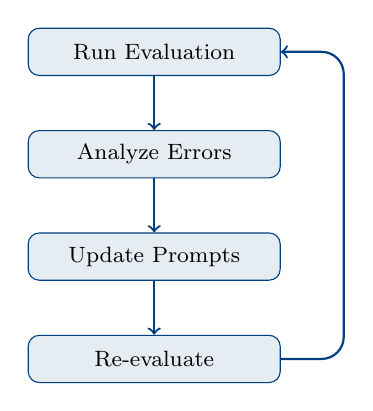
\begin{tikzpicture}[
        box/.style={rectangle, draw=upcblue, fill=upcblue!10, rounded corners, minimum width=3.2cm, minimum height=0.6cm, align=center, font=\footnotesize},
        arrow/.style={->, thick, upcblue}
      ]
        \node[box] at (0, 0)    (eval)   {Run Evaluation};
        \node[box] at (0, -1.3) (analyze){Analyze Errors};
        \node[box] at (0, -2.6) (update) {Update Prompts};
        \node[box] at (0, -3.9) (test)   {Re-evaluate};
        
        \draw[arrow] (eval) -- (analyze);
        \draw[arrow] (analyze) -- (update);
        \draw[arrow] (update) -- (test);
        \draw[arrow, rounded corners=8pt] (test.east) -- ++(0.8,0) -- ++(0,3.9) -- (eval.east);
      \end{tikzpicture}
    \end{column}
  \end{columns}
  \note{The LLM-as-judge framework enabled iterative prompt refinement. A coding agent analyzed evaluation failures and updated the system prompt accordingly. This agentic optimization loop is becoming standard practice.}
\end{frame}

% =============================================================================
% SLIDE 10: Question Categories & Metrics
% =============================================================================
\begin{frame}{Evaluation Dataset \& Metrics}
  \begin{columns}[T,onlytextwidth]
    \begin{column}{0.48\textwidth}
      \textbf{Question Categories}
      \vspace{0.3em}
      \begin{table}
        \footnotesize
        \begin{tabular}{lr}
          \toprule
          Category & Count \\
          \midrule
          courses & 13 \\
          exams & 5 \\
          professors & 4 \\
          personal (OAuth) & 4 \\
          multi\_tool & 5 \\
          ambiguous & 4 \\
          news, academic, etc. & 10 \\
          \bottomrule
        \end{tabular}
      \end{table}
      \vspace{0.3em}
      \textbf{Complexity:} Simple, Multi-step, Contextual, Ambiguous
    \end{column}
    \begin{column}{0.48\textwidth}
      \textbf{7 Evaluation Metrics}
      \vspace{0.3em}
      \begin{itemize}
        \item \textbf{Relevance} -- addresses the question?
        \item \textbf{Helpfulness} -- actionable \& useful?
        \item \textbf{Conciseness} -- appropriately brief?
        \item \textbf{Structure} -- well-organized?
        \item \textbf{Tone} -- professional?
        \item \textbf{Error Handling} -- graceful failures?
        \item \textbf{Tool Appropriateness} -- right tools?
      \end{itemize}
    \end{column}
  \end{columns}
  \note{Our dataset covers 10 categories and 4 complexity levels. Each response is scored on 7 metrics with detailed rubrics defining correct and incorrect behaviors.}
\end{frame}

% =============================================================================
% SLIDE 11: Results - The Numbers
% =============================================================================
\begin{frame}{Results: Model Comparison}
  \begin{table}
    \scriptsize
    \centering
    \begin{tabular}{lcccccc}
      \toprule
      Metric & Target & \textbf{Gemini 3 Flash} & \textbf{Gemini 2.5 Flash} & \textbf{Gemini 2.5 Pro} & \textbf{Qwen 7B} & \textbf{Llama 3B} \\
      \midrule
      Relevance & $>$0.85 & \textcolor{green!60!black}{0.98} & \textcolor{green!60!black}{0.90} & \textcolor{green!60!black}{0.89} & \textcolor{red!70!black}{0.74} & \textcolor{red!70!black}{0.22} \\
      Helpfulness & $>$0.85 & \textcolor{green!60!black}{0.99} & \textcolor{green!60!black}{0.89} & \textcolor{green!60!black}{0.93} & \textcolor{red!70!black}{0.80} & \textcolor{red!70!black}{0.32} \\
      Conciseness & $>$0.80 & \textcolor{green!60!black}{0.87} & \textcolor{green!60!black}{0.85} & \textcolor{green!60!black}{0.83} & \textcolor{red!70!black}{0.69} & \textcolor{red!70!black}{0.28} \\
      Structure & $>$0.75 & \textcolor{green!60!black}{0.79} & \textcolor{green!60!black}{0.77} & \textcolor{green!60!black}{0.80} & \textcolor{green!60!black}{0.76} & \textcolor{red!70!black}{0.29} \\
      Tone & $>$0.80 & \textcolor{green!60!black}{0.89} & \textcolor{green!60!black}{0.85} & \textcolor{green!60!black}{0.85} & \textcolor{green!60!black}{0.81} & \textcolor{red!70!black}{0.37} \\
      Error Handling & $>$0.70 & \textcolor{green!60!black}{0.74} & \textcolor{red!70!black}{0.51} & \textcolor{red!70!black}{0.43} & \textcolor{red!70!black}{0.29} & \textcolor{red!70!black}{0.08} \\
      Tool Approp. & $>$0.80 & \textcolor{orange!80!black}{0.75} & \textcolor{orange!80!black}{0.77} & \textcolor{orange!80!black}{0.78} & \textcolor{red!70!black}{0.43} & \textcolor{red!70!black}{0.09} \\
      \midrule
      \textbf{Average} & & \textbf{0.86} & \textbf{0.79} & \textbf{0.79} & \textbf{0.65} & \textbf{0.24} \\
      \bottomrule
    \end{tabular}
  \end{table}
  \vspace{0.3em}
  \textbf{Key Findings}
  \begin{itemize}
    \item Gemini 3 Flash: best overall (0.86 avg), only model to pass error handling
    \item Gemini 2.5 models: solid performance, Flash \& Pro nearly identical
    \item Open-source: Qwen 7B reasonable (0.65), Llama 3B insufficient (0.24)
  \end{itemize}
  \note{Gemini 3 Flash shows significant improvement, especially in error handling (0.74 vs 0.51). Clear performance gap between proprietary and open-source models. Qwen shows promise but struggles with tool use.}
\end{frame}

% =============================================================================
% SLIDE 12: Lessons Learned
% =============================================================================
\begin{frame}{Lessons Learned}
  \begin{columns}[T,onlytextwidth]
    \begin{column}{0.52\textwidth}
      \textbf{Challenges \& Solutions}
      \vspace{0.5em}
      \begin{itemize}
        \item \textbf{Ambiguous queries}
        \begin{itemize}
          \item[$\rightarrow$] Present top matches first
          \item[$\rightarrow$] Then ask for clarification
        \end{itemize}
        \vspace{0.3em}
        \item \textbf{Date-relative queries}
        \begin{itemize}
          \item[$\rightarrow$] Explicit date in context
          \item[$\rightarrow$] Weekday mappings in prompt
        \end{itemize}
        \vspace{0.3em}
        \item \textbf{Error handling scored low}
        \begin{itemize}
          \item[$\rightarrow$] Rubric was overly strict
          \item[$\rightarrow$] Agent too verbose on errors
        \end{itemize}
        \vspace{0.3em}
        \item \textbf{Tool tracking across subagents}
        \begin{itemize}
          \item[$\rightarrow$] Evaluation sees only ``task'' call
          \item[$\rightarrow$] Need trajectory flattening
        \end{itemize}
      \end{itemize}
    \end{column}
    \begin{column}{0.45\textwidth}
      \centering
      \includegraphics[width=\linewidth,height=0.75\textheight,keepaspectratio]{assets/s12_lessons.png}
    \end{column}
  \end{columns}
  \note{Key lessons: handle ambiguity by offering options first, provide date context explicitly, and be aware that hierarchical architectures complicate tool tracking in evaluation.}
\end{frame}

% =============================================================================
% SLIDE 13: Contributions & Future Work
% =============================================================================
\begin{frame}{Contributions \& Future Work}
  \begin{columns}[T,onlytextwidth]
    \begin{column}{0.52\textwidth}
      \small
      \textbf{Contributions}
      \vspace{0.2em}
      \begin{itemize}
        \setlength{\itemsep}{0.1em}
        \item Open-source FIB Agent with hierarchical architecture
        \item 45-question evaluation dataset (10 categories)
        \item Reusable LLM-as-judge framework
        \item MCP server for AI interoperability
        \item Documented prompt engineering patterns
      \end{itemize}
      \vspace{0.3em}
      \textbf{Future Directions}
      \vspace{0.2em}
      \begin{itemize}
        \setlength{\itemsep}{0.1em}
        \item RAG with syllabi \& lecture notes
        \item Conversation memory (multi-turn)
        \item User interface (Telegram bot, web chat)
        \item Multi-university adaptation
      \end{itemize}
    \end{column}
    \begin{column}{0.45\textwidth}
      \centering
      \includegraphics[width=\linewidth,height=0.75\textheight,keepaspectratio]{assets/s13_future.png}
    \end{column}
  \end{columns}
  \note{Our contributions include the agent, dataset, evaluation framework, and MCP server. Future work includes RAG for richer answers, conversation memory, and user-facing interfaces.}
\end{frame}

% =============================================================================
% SLIDE 14: Thank You / Q&A
% =============================================================================
\begin{frame}{Thank You}
  \begin{columns}[T,onlytextwidth]
    \begin{column}{0.55\textwidth}
      \vspace{1em}
      \textbf{Key Takeaway}
      \vspace{0.5em}
      \begin{quote}
        ``Modern LLM agents can effectively serve as natural language interfaces to structured APIs when properly configured with domain-specific tools and engineered prompts.''
      \end{quote}
      \vspace{1em}
      \textbf{Links}
      \begin{itemize}
        \item GitHub: \url{https://github.com/akossch0/upc-fib-agent}
        \item FIB API: \url{https://api.fib.upc.edu/v2/}
        \item LangGraph: \url{https://langchain-ai.github.io/langgraph/}
      \end{itemize}
      \vspace{1em}
      \centering
      \Large Questions?
    \end{column}
    \begin{column}{0.42\textwidth}
      \centering
      \includegraphics[width=\linewidth,height=0.75\textheight,keepaspectratio]{assets/s14_thankyou.png}
    \end{column}
  \end{columns}
  \note{Thank you for your attention. The key message is that LLM agents with proper tooling and prompts can serve as effective natural language interfaces. Happy to take questions!}
\end{frame}

\end{document}
